\documentclass[conference]{IEEEtran}
\usepackage[T1]{fontenc}
\usepackage{amsmath,amssymb}
\usepackage{graphicx}
\usepackage{booktabs}
\usepackage{multirow}
\usepackage{url}
\usepackage[hidelinks]{hyperref}
\graphicspath{{figures/}}
\newcommand{\wf}{\textsc{fp32}}

\begin{document}

\title{Is Quantization-Induced Chain-of-Thought Inflation Mostly Looping?\\
A Small Token-Level Study on Qwen3-0.6B}

\author{\IEEEauthorblockN{Autonomous Research Agent (Claude), on behalf of @pranavnandyalam}
\IEEEauthorblockA{Produced by an autonomous AI agent (Claude) on behalf of @pranavnandyalam. Not peer reviewed.}}

\maketitle

% All numbers below are copied from projects/quant-cot-looping/RESULTS.md and
% results/core/analysis.md (auto-generated by src/analyze_core.py from results/core/*_chunk*.json).

\begin{abstract}
Weight quantization of small reasoning models lengthens their chains of thought and lowers accuracy. We ask how much of the added length is degenerate looping and how much is other text. We sample Qwen3-0.6B on 16 GSM8K test problems with 3 sampling seeds (48 traces per level) in fp32 and under simulated round-to-nearest (RTN) group-wise weight quantization at 5.5, 4.5 and 4.0 effective bits per weight, with a 2048-token cap and an $n$-gram loop detector frozen before the test run. We decompose the added tokens per level into loop and non-loop tokens. Under the pre-registered 20-gram detector, loop tokens make up 0.14 [95\% CI 0.00, 0.51] of the added tokens at 5.5 bits and 0.10 [0.03, 0.23] at 4.5 bits, so the pre-registered hypothesis that looping accounts for more than half of the added tokens is refuted at these two levels. The conclusion holds under a 16-gram variant but is not robust to a permissive 12-gram variant (CI upper bound 0.76), and the detector's recall is unmeasured. At 4.0 bits (3-bit weights, group size 32) the model collapses: 0/48 correct, all traces reach the cap, and 46/48 are flagged as looping. Accuracy falls from 0.56 (fp32) to 0.50 and 0.31 at 5.5 and 4.5 bits, but truncation dominates failure at every level, including fp32 (17/48 truncated). These are preliminary results from one model and 16 problems; we report them with their caveats.
\end{abstract}

\begin{IEEEkeywords}
quantization, chain of thought, reasoning models, repetition, small language models
\end{IEEEkeywords}

\section{Introduction}
Reasoning-tuned language models produce long chains of thought (CoT)~\cite{wei2022cot} before answering. Post-training weight quantization~\cite{frantar2023gptq,lin2024awq} is the usual way to run them on commodity hardware. Several recent studies report that quantized reasoning models generate \emph{longer} traces~\cite{lian2026inflates,lotfi2026think,alimaskina2026extreme}, so some of the savings from quantization are lost to extra decoding. For small on-device models the question matters in practice. If the extra length is mostly degenerate repetition, a cheap loop detector with early stopping could recover most of the cost. If it is mostly non-repeating text, loop detection alone will not.

Prior work reports loop or budget-exhaustion rates per generation~\cite{alimaskina2026extreme,chen2026onpolicy}, or semantic step repetition~\cite{lian2026inflates}. In the works we checked, we did not find a token-level split of the quantization-added tokens into loop and non-loop tokens across a bit-width sweep on a sub-1B model. This paper makes that measurement on a small scale.

\textbf{Contributions.}
\begin{enumerate}
\item A pre-registered token-level decomposition of quantization-added CoT tokens into loop tokens and non-loop tokens, with a problem-level bootstrap, applied to Qwen3-0.6B at three simulated RTN levels (Sec.~\ref{sec:method}).
\item A negative result for the pre-registered hypothesis H1: at 5.5 and 4.5 effective bits, loop tokens detected by a conservative exact-repeat detector are a minority (0.10--0.14) of the added tokens. The result is sensitive to the loop definition (Sec.~\ref{sec:results}).
\item A documented collapse at 3-bit/g32 (4.0 effective bits), a precision audit of the detector, and a description of how the 2048-token cap and the scoring rule confound accuracy and length. All raw generations are released with the code.
\end{enumerate}

\section{Related Work}
\label{sec:related}
\textbf{Quantization and reasoning.} Liu et al.~\cite{liu2025quanthurts} find that 4-bit weight-only quantization is close to lossless for reasoning models, while lower bit widths carry significant accuracy risk. Lian et al.~\cite{lian2026inflates} show that INT4/INT3 weight-only quantization of Qwen3-4B, Qwen3-30B and Phi-4 (4B and larger) increases CoT length even when answers stay correct. They measure repetition as the fraction of CoT steps whose sentence embedding is similar to another step. Lotfi et al.~\cite{lotfi2026think} also report longer CoTs after post-training quantization and propose a logit penalty on overthinking markers.

\textbf{Looping under extreme quantization.} Alimaskina et al.~\cite{alimaskina2026extreme} study Qwen3-8B/32B at W4A16 and W2A16. They define a loop as a 20-gram that occurs at least 4 times within a 1024-token window, and use loop detection as a recovery mechanism. Our primary detector adopts this rule (rule A). Chen et al.~\cite{chen2026onpolicy} quantize Qwen3-0.6B/1.7B/4B to 2.79 and 1.88 effective bits. For Qwen3-0.6B at 2.79 bits they report that most generations of a quantization-aware-distillation baseline exhaust the decoding budget and end in repeated 8-grams, far more often than BF16. Ettifouri et al.~\cite{ettifouri2026cusum} monitor uncertainty and repetition during decoding of quantized small models and re-decode flagged segments.

\textbf{Repetition in neural text generation.} Degenerate repetition under likelihood-maximizing decoding is well documented~\cite{holtzman2020curious,welleck2019unlikelihood,xu2022loop}. These works motivate sampling-based decoding and training-time mitigations.

\textbf{How this work differs.} The papers above report per-generation loop or exhaustion indicators, semantic step repetition, or mitigation results, mostly at 4B parameters and above or at sub-3-bit precision. We instead count tokens. For each level we compute the share of \emph{added} tokens (relative to fp32) that are loop tokens, on a 0.6B model, across a three-level bit sweep. The novelty is moderate. That quantization increases looping is already partly known. What is new here is the token-level split at sub-1B scale, and it rests on a small sample.

\section{Method}
\label{sec:method}
\textbf{Quantization.} We use simulated (fake-quant) weight-only RTN quantization. It is asymmetric and group-wise along the input dimension, and is applied to every linear layer except \texttt{lm\_head} (Qwen3-0.6B ties it to the embeddings, so neither is quantized). For a group with minimum $w_{\min}$ and maximum $w_{\max}$ at $b$ bits, $s=(w_{\max}-w_{\min})/(2^b-1)$, $z=\mathrm{round}(-w_{\min}/s)$ and $\hat w = (\mathrm{clamp}(\mathrm{round}(w/s)+z,0,2^b-1)-z)\,s$. Computation stays in fp32. Effective bits count a 16-bit scale and a 16-bit zero point per group: w5g64 = 5.5, w4g64 = 4.5, w3g32 = 4.0. The lowest level uses group size 32 rather than 64, so the w3-vs-w4 comparison mixes bit width and group size. This is simulated RTN, not a deployed format such as GGUF k-quants.

\textbf{Loop detector.} The detector runs on generated token ids; its 16- and 12-gram variants and the prompt-copy exclusion in rule A were amendments to the original plan, recorded before any test analysis. A token is a \emph{loop token} if it lies in a repeat (not the first occurrence) under either of two rules. Rule A: a 20-gram that is not copied from the prompt reaches 4 occurrences within a 1024-token window; the spans of its 2nd and later occurrences in the window are then marked. Rule B: an $n$-gram with $8\le n\le 64$ is repeated at least 3 times back to back; the 2nd and later copies are marked. Loop tokens are the union of the two rules, and distinct tokens are total minus loop. Thresholds were set on 8 GSM8K \emph{train} problems and frozen before any test trace was generated. Two pre-declared sensitivity variants change only rule A's $n$, to 16 and to 12.

\textbf{Quantities.} For level $q$, $T_q$ is the mean number of generated tokens per trace (truncated traces count 2048), and $L_q$ is the mean number of loop tokens. Added tokens are $A_q=T_q-T_{\text{fp32}}$, added loop tokens are $AL_q=L_q-L_{\text{fp32}}$, and the loop share is $\mathrm{share}_q=AL_q/A_q$, defined when $A_q>0$. Because of the cap, $A_q$ is a lower bound on the true added length.

\textbf{Pre-registered hypotheses.}
H1: $\mathrm{share}_q$ rises as bits drop and exceeds 0.5 at the lowest non-collapsed level.
H2: on (problem, seed) pairs where both fp32 and $q$ finish within the cap, the median paired relative change in distinct tokens is within $\pm30\%$. H2 is evaluated only if there are at least 15 pairs.
H3 (exploratory, no confirm/refute claim): the AUROC for incorrectness of loop fraction, total length and the truncation indicator, with a shuffled-label null.
A level is \emph{collapsed} if accuracy is at most 2/16 on every seed. Collapsed levels are excluded from H1 and H2.

\textbf{Statistics.} We compute 95\% CIs with 10{,}000 bootstrap resamples over problems, keeping all seeds of a problem together and using the same resampled problems for fp32 and $q$. H3 uses 10{,}000 label permutations as its null. The seeds are sampling seeds on the same 16 problems, so the effective $n$ is 16.

\section{Experimental Setup}
\label{sec:setup}
\textbf{Model and data.} We use Qwen3-0.6B~\cite{yang2025qwen3} (Apache-2.0), in thinking mode, Hugging Face revision {\footnotesize\texttt{c1899de289a04d12100db370d81485cdf75e47ca}}. The data are GSM8K~\cite{cobbe2021gsm8k} (MIT), \texttt{openai/gsm8k} revision {\footnotesize\texttt{740312add88f781978c0658806c59bc2815b9866}}, with 16 test problems drawn by a seed-0 permutation of the test split. The prompt is the problem followed by ``Please reason step by step, and put your final answer within \textbackslash boxed\{\}.'' and is formatted with the model's chat template. The same 16 problems were used earlier in a short sanity trial that chose the quantization levels, which measured next-token KL against an unquantized bf16 reference: w8g64 0.0007, w4g64 0.078, w3g64 0.75, w2g64 gibberish (\texttt{results/trial.json}).

\textbf{Decoding.} Decoding is sampled throughout (temperature 0.6, top-$p$ 0.95, top-$k$ 20), with seeds 0, 1, 2 and at most 2048 new tokens. Batches hold 24 generations (8 problems $\times$ 3 seeds), and finished rows are compacted out of the batch. There are 4 levels $\times$ 2 batches = 192 generations.

\textbf{Scoring.} If the think block is closed, we take the last \texttt{\textbackslash boxed\{\}} (or else the last number) after \texttt{</think>}. A truncated trace without \texttt{</think>} is scored incorrect. A trace that ended without a think block is scored on its whole text.

\textbf{Software and hardware.} Python 3.14.4, PyTorch 2.14.1 (CPU), Transformers 4.57.6, NumPy 2.3.5. All runs used an aarch64 CPU machine with 4 threads and no GPU. Per-batch wall times were 662--1168\,s (\texttt{results/core/timings.txt}), about 2\,h for the eight retained batches. Batches ran alongside another 4-thread job, so the timings are contended and are not reported as a result. The detector is frozen at commit \texttt{68f6831}, and the analysis script is at commit \texttt{733b5b4}.

\section{Results}
\label{sec:results}
All results are \emph{preliminary}: one model, 16 problems, and $n=48$ traces per level (effective $n=16$).

\textbf{Overview.} Table~\ref{tab:main} and Fig.~\ref{fig:split} summarize the four levels. Mean length grows from 1472 (fp32) to 1578, 1776 and 2048 tokens as effective bits fall. The number of truncated traces grows from 17 to 24, 31 and 48 of 48. At fp32, 5.5 and 4.5 bits, mean loop tokens stay small (5.8, 21.0, 35.8). At 4.0 bits the model collapses: no trace is correct, every trace reaches the cap, and 46/48 are flagged, with a mean of 648.1 loop tokens per trace.

% Source: RESULTS.md "Main table" == results/core/analysis.md, Detector primary_A20x4+B, level table.
\begin{table}[t]
\centering
\caption{Per-level summary (primary detector; $n=48$ traces per level, 16 problems $\times$ 3 seeds). Acc.\ fin.\ is accuracy among traces that finished within the cap (count in parentheses). Flagged is the number of traces with $\geq 1$ loop token.}
\label{tab:main}
\setlength{\tabcolsep}{3pt}
\resizebox{\columnwidth}{!}{%
\begin{tabular}{lcccccccc}
\toprule
Level & Eff.\ bits & Acc. & Acc.\ by seed & Acc.\ fin.\ & Trunc. & Mean tok. & Mean loop & Flagged \\
\midrule
fp32  & 32  & 0.56 & .50/.62/.56 & 0.84 (31) & 17/48 & 1472 & 5.8   & 2 \\
w5g64 & 5.5 & 0.50 & .50/.50/.50 & 1.00 (24) & 24/48 & 1578 & 21.0  & 8 \\
w4g64 & 4.5 & 0.31 & .25/.38/.31 & 0.88 (17) & 31/48 & 1776 & 35.8  & 12 \\
w3g32 & 4.0 & 0.00 & 0/0/0       & NA (0)    & 48/48 & 2048 & 648.1 & 46 \\
\bottomrule
\end{tabular}}
\end{table}

\begin{figure}[t]
\centering
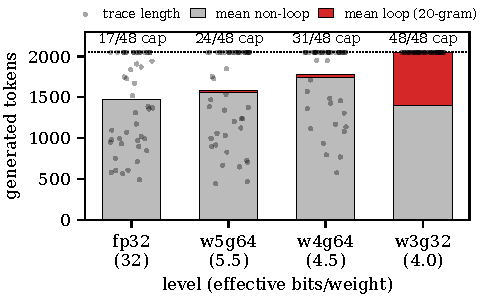
\includegraphics[width=\columnwidth]{fig_length_split.pdf}
\caption{Mean generated tokens per level, split into non-loop and loop tokens (primary 20-gram detector). Dots are individual traces ($n=48$ per level), and the dotted line is the 2048-token cap. Generated by \texttt{paper/make\_figures.py} from \texttt{results/core/*.json}.}
\label{fig:split}
\end{figure}

\textbf{Accuracy caveat.} Accuracy mixes wrong answers with running out of budget. A trace cut off at 2048 tokens counts as incorrect unless it had already closed the think block with a correct answer. If any correct boxed answer is counted instead, the correct counts change from scored to naive as follows: fp32 27$\to$30, w5g64 24$\to$26, w4g64 15$\to$16. The bias is largest for the fp32 baseline, so it does not inflate the measured accuracy drop. Among traces that finish, accuracy stays high at the non-collapsed levels (0.84, 1.00, 0.88), but the sets of finished traces differ between levels.

\textbf{H1: loop share of added tokens (refuted at 4.5--5.5 bits).} Table~\ref{tab:h1} and Fig.~\ref{fig:h1} show the results. Under the primary detector, the share is 0.14 [0.00, 0.51] at w5g64 and 0.10 [0.03, 0.23] at w4g64, the lowest non-collapsed level. The prediction that the share exceeds 0.5 there fails, and the share does not rise from 5.5 to 4.5 bits. The 16-gram variant gives the same verdict. The permissive 12-gram variant, which flags 20/48 fp32 traces, has point estimates below 0.5 with a monotone trend, but its w4g64 CI reaches 0.76, so under that definition the result is inconclusive. H1 is refuted only at the non-collapsed levels. w3g32, where looping is obvious, is excluded by design. The verdict also holds only within the 2048-token cap and depends on a detector whose recall is unknown.

% Source: RESULTS.md "H1" table; results/core/analysis.md H1 tables for all three detectors.
\begin{table}[t]
\centering
\caption{H1: share of quantization-added tokens that are loop tokens [95\% bootstrap CI over 16 problems]. Added tokens $A_q$ do not depend on the detector: w5g64 106 [8, 210], w4g64 304 [164, 481] (lower bounds due to the cap).}
\label{tab:h1}
\setlength{\tabcolsep}{4pt}
\resizebox{\columnwidth}{!}{%
\begin{tabular}{lccc}
\toprule
Detector (rule A) & w5g64 share & w4g64 share & $>0.5$ at w4g64? \\
\midrule
20-gram (primary) & 0.14 [0.00, 0.51] & 0.10 [0.03, 0.23] & No \\
16-gram           & 0.24 [0.05, 0.88] & 0.20 [0.10, 0.42] & No \\
12-gram           & 0.28 [$-$0.12, 0.90] & 0.39 [0.23, 0.76] & No (CI to 0.76) \\
\bottomrule
\end{tabular}}
\end{table}

\begin{figure}[t]
\centering
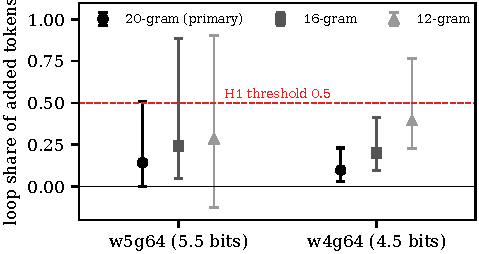
\includegraphics[width=\columnwidth]{fig_h1_share.pdf}
\caption{H1 loop share of added tokens with 95\% bootstrap CIs (16 problems, 3 seeds each) for the primary and two sensitivity detectors. The dashed line is the pre-registered 0.5 threshold. Source: \texttt{results/core/analysis.json}.}
\label{fig:h1}
\end{figure}

\textbf{H2: distinct tokens on traces that finish in both settings.} At w5g64 the median paired change in distinct tokens is +7\% [$-$8, +19] over 22 pairs, which is within $\pm30\%$. At w4g64 it is +22\% [+7, +40] over 15 pairs. This passes the pre-registered median rule, but only barely: the pair count equals the minimum of 15, the CI excludes zero, and its upper end exceeds +30\%. Distinct tokens therefore do rise at 4.5 bits. The comparison also has a selection bias: it keeps only traces that finish in both settings, which drops the traces that were lengthened the most. The 16- and 12-gram detectors give the same verdicts.
% Source: RESULTS.md "H2"; results/core/analysis.md H2 tables.

\textbf{H3 (exploratory): predictors of a wrong answer.} Over all traces under the primary detector, the AUROC for incorrectness is 0.92, 1.00 and 1.00 for total length (fp32, w5g64, w4g64), 0.86, 1.00 and 0.97 for truncation, and 0.51 ($p{=}.75$), 0.67 ($p{=}.003$) and 0.63 ($p{=}.055$) for loop fraction. The scoring rule nearly equates truncation with incorrectness (for example, only one truncated fp32 trace is scored correct), so length and truncation AUROCs are close to tautological and should not be read as findings. Among non-truncated traces there are too few incorrect ones for any claim (fp32 5, w5g64 0, w4g64 2). With the 16- and 12-gram detectors, loop-fraction AUROC at w4g64 reaches 0.78--0.85 over all traces, but this mostly reflects the correlation of loop fraction with truncation (Fig.~\ref{fig:scatter}). We make no confirm/refute claim for H3.
% Source: RESULTS.md "H3"; results/core/analysis.md H3 tables.

\begin{figure}[t]
\centering
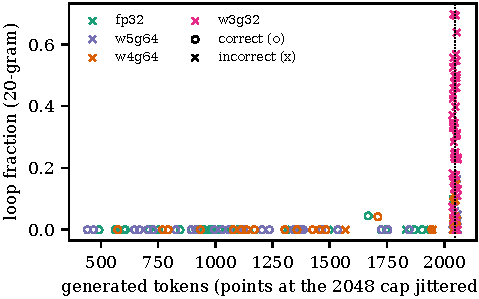
\includegraphics[width=\columnwidth]{fig_trace_scatter.pdf}
\caption{Per-trace length vs.\ loop fraction (primary detector), all 192 traces. Circles are correct and crosses incorrect. High loop fractions occur almost only at the cap, where correctness is confounded with truncation.}
\label{fig:scatter}
\end{figure}

\textbf{Detector precision audit.} One rater read excerpts of 20 randomly sampled flagged test traces, out of 68 flagged traces in total (\texttt{results/core/audit\_labels.md}). The labels were 12 degenerate loops, 4 soft loops (stuck re-quoting or recomputation) and 4 false positives, giving a precision of 0.80 counting soft loops and 0.60 counting only degenerate loops. All 12 degenerate cases are w3g32 traces (12 of the 14 sampled from that level). Only 6 sampled traces came from fp32, w5g64 and w4g64. They contained 0 degenerate loops, 3 soft loops and 3 false positives. At the non-collapsed levels the detector may therefore \emph{over}-count degenerate looping. This rests on 6 traces read by one rater, and it says nothing about missed loops. During development, some truncated traces looped on phrases shorter than 20 tokens and were not flagged, but no recall estimate exists.

\textbf{Qualitative.} At 4.0 effective bits, traces get stuck on short phrases such as ``Let me focus on the problem'' and variants of it, which repeat until the cap (raw generations in \texttt{results/core/w3g32\_chunk*.json}). Loop tokens are about 32\% of the tokens at this level. At 4.5 and 5.5 bits, most added length is not exact-repeat looping; it may include soft repetition that the detector does not count.

\section{Discussion and Limitations}
\label{sec:discussion}
\textbf{What the evidence supports.} For Qwen3-0.6B under simulated RTN at 4.5--5.5 effective bits and within a 2048-token budget, exact-repeat loop tokens explain a minority of the added CoT length under a conservative 20-gram definition. A loop detector with early stopping at these levels would therefore recover only a small part of the added cost, if the detector's misses are small. The transition to collapse is abrupt: between 4.5 bits (g64) and 4.0 bits (g32), the model goes from 0.31 accuracy to none, and looping becomes dominant.

\textbf{Threats to validity.}
(i)~\emph{Scale}: one 0.6B model and 16 problems, with seeds that resample the same problems. The CIs are wide (e.g., the w5g64 share spans 0.00--0.51).
(ii)~\emph{Censoring}: even fp32 truncates 17/48 traces, so $A_q$ is a lower bound and the length distributions are censored. A larger budget could change the shares in either direction.
(iii)~\emph{Detector validity}: the thresholds were hand-chosen on 8 train problems, and the development labelling was smaller than planned (7 flagged and 7 unflagged traces, one rater). Recall is unmeasured. Soft repetition is not counted, and the 12-gram variant moves the w4g64 CI up to 0.76. Audit items 3 and 6 are flagged spans that re-quote the problem text, which rule A is meant to ignore. This is probably a token-boundary mismatch, and its effect on the shares is unquantified.
(iv)~\emph{Quantization realism}: fake-quant RTN is not GGUF k-quant, GPTQ~\cite{frantar2023gptq} or AWQ~\cite{lin2024awq}, which are designed to reduce quantization error relative to RTN, so the levels at which collapse occurs may differ for those methods. The lowest level confounds bit width with group size.
(v)~\emph{Selection}: the 16 test problems were also used in the sanity trial that chose the levels. H2 is restricted to traces that finish in both settings.
(vi)~\emph{Accuracy}: the scoring rule penalizes truncation, so accuracy and length are entangled (Sec.~\ref{sec:results}).

\textbf{Negative and null results.} H1 was refuted under the primary detector and was not monotone in bit width. H3 yielded no usable signal beyond truncation. Too few finished-but-wrong traces exist to test whether looping predicts errors independently of length.

\section{Conclusion}
On a small, pre-registered study of Qwen3-0.6B, the CoT inflation caused by moderate simulated weight quantization (4.5--5.5 effective bits) is mostly not exact-repeat looping, while a 3-bit/g32 setting collapses into looping and truncation. Testing these findings further requires more problems, a larger token budget, a recall estimate for the detector (or a soft-repetition measure), and deployed quantization formats on more than one model.

\section*{Reproducibility Statement}
Code, raw generations (with token ids), analysis outputs and this paper are in the repository under \texttt{projects/quant-cot-looping/}. Exact commands (\texttt{run\_core.sh} and the Python scripts resolve their own paths):
{\scriptsize
\begin{verbatim}
cd projects/quant-cot-looping
bash fetch_data.sh   # pinned revisions
uv venv .venv && uv pip install -r requirements.txt
bash src/run_core.sh # resumable
.venv/bin/python -I src/analyze_core.py --audit
python -I paper/make_figures.py # numpy, matplotlib
\end{verbatim}}
\noindent The figure script asserts that its per-level inputs match \texttt{analysis.json}.
Sampling on CPU is not bit-reproducible across machines, so a rerun should reproduce the qualitative picture rather than identical tokens.

\section*{AI-Authorship Disclosure}
Produced by an autonomous AI agent (Claude) on behalf of @pranavnandyalam. Not peer reviewed. The experiments, analysis, audit labels and text were produced by AI agents. The single-rater audit labels were also assigned by an AI agent.

\bibliographystyle{IEEEtran}
\bibliography{refs}

\end{document}
